%!TEX root = ../thesis.tex
\section{Service: Entwurf und Implementierung}

Der Service ist der Antrieb des gesamten Systems. In ihm werden Daten berechnet und persistiert. Wie im Architekturentwurf (\fullref{sec:architektur}) schon beschrieben, besitzt der Service eine \ac{API}. Das ist nichts besonderes: ein Webservice definiert sich darüber, dass er eine maschinenlesbare Schnittstelle besitzt.

Eine Besonderheit im Webservice von WARP ist die Pipeline. Sie wird ebenfalls vom Service ausgeführt. Daher beschäftigt sich dieser Abschnitt zwar auch mit der \ac{API}, aber vor allem mit dem Entwurf und der Implementierung der Build-Pipeline.

\subsection{Elixir und Phoenix}

Bei Webanwendungen hängt (wie in anderen Domänen auch) die Wahl einer Programmiersprache des Webservices weniger davon ab, welches Problem die Anwendung lösen soll, sondern mehr von der Erfahrung der im Projekt beteiligten Entwickler ab. Die Auswahl an serverseitigen Programmiersprachen ist groß, und jede Programmiersprache besitzt ihre eigenen Vorteile.

Die Wahl der Programmiersprache fiel für dieses Projekt auf \textbf{Elixir}.

Elixir wurde 2011 von José Valim veröffentlicht und ist somit eine relativ junge Programmiersprache. Elixir basiert auf Erlang, einer seit 1986 von Ericsson entwickelten Programmiersprache und Laufzeitumgebung. Das Erlang System ist u.a. für seine hohe Verfügbarkeit bekannt, es kann auf vielen Servern parallel laufen, und aktualisiert werden ohne die Anwendung stoppen zu müssen. Die Programmiersprache Erlang ist funktional, weshalb Elixir ebenfalls eine funktionale Programmiersprache ist.

Elixir wurde nicht gewählt, da darin schon Erfahrung besteht, sondern um Erfahrung in Elixir zu erlangen: Zu Beginn der Arbeit waren weder Kenntnisse in Elixir noch in Erlang vorhanden.

Als Webframework für Elixir wurde das bekannteste Framework gewählt: \textbf{Phoenix}.

Phoenix ist ein Framework für Webanwendungen nach dem \ac{MVC} Modell. Es beinhaltet viele nützliche Bestandteile wie eine Datenbank-Abstraktion (ähnlich zu einem \acs{ORM}\footnote{\acf{ORM}. da Elixir eine funktionale Programmiersprache ist und somit keine Objekte besitzt, ist der Begriff \acs{ORM} nicht zutreffend, jedoch vergleichbar mit ORMs aus anderen Sprachen.}) und eine einfache Implementierung von Websockets, welche im weiteren Verlauf der Arbeit zur Echtzeitkommunikation benötigt werden.

\subsection{Entwurf einer RESTful API}

\ac{REST} ist ein von Roy Fielding entworfener Architekturstil für ``verteilte Hypermedia Systeme''. Fielding nennt grundlegend zwei Bedingungen für ein solches System:

\begin{itemize}
  \item Die Trennung des Systems in eine Client-Server Architektur. Dies folgt dem Prinzip der ``Trennung der Belange'' (Separation of Concerns), und teilt die Anwendung in die Nutzeroberfläche (Client) die Datenverwaltung (Server).
  \item Die Kommunikation zwischen Client und Server ist zustandslos (stateless). Der Client muss dem Server alle Daten übermitteln, die der Server zum Verständnis und Ausführen der Anfrage benötigt.\footnote{Im Gegensatz zu Sessions, bei denen auf dem Server Informationen zu jedem Client gespeichert werden.}
\end{itemize}

Alle Interaktionen mit dem Service bestehen aus dem Aufruf einer Ressource, einem Identifikator und einer Aktion \citep[12]{Webber2010}. \ac{REST} ist kein Standard, daher kann sich die Implementierung von \ac{REST}\footnote{Wenn wir REST implementieren, verwenden wir die Adjektivform \emph{``RESTful''}.} von Fall zu Fall unterscheiden. Bei Webanwendungen werden meist mindestens folgende Informationen aus dem \ac{HTTP} Protokol genutzt:

\begin{itemize}
  \item Der Pfad der \acs{URL} bestimmt die Ressource und den Identifikator.
  \item Die \ac{HTTP} Methode bestimmt die auszuführende Aktion.
\end{itemize}

In Richardsons Maturity Model entspricht dies einem Level Two Service (vgl. \citep[20]{Webber2010}). Dabei werden auch HTTP Statuscodes genutzt, um dem Client einen standardisierten Status der Anfrage zu übermitteln.

Für den Service wurden die in \tabref{tab:rest-routes} definierten Endpunkte für eine RESTful API ausgearbeitet. Als Datenformat wurde JSON gewählt, da sich dies sich besonders für die Verwendung in einem JavaScript-basierten Frontend Client eignet.

\begin{table}[H]
  \footnotesize
  \begin{tabularx}{\textwidth}{| l | l | X |}
    \hline
    \textbf{Verb} & \textbf{Pfad} & \textbf{Beschreibung} \\ \hline
    GET & {\scriptsize \texttt{/projects}} & Auflisten aller Projekte \\ \hline
    POST & {\scriptsize \texttt{/projects}} & Erstellen eines neuen Projekts \\ \hline
    GET & {\scriptsize \texttt{/projects/:project\_id}} & Auslesen eines Projekts anhand seiner ID \\ \hline
    PUT & {\scriptsize \texttt{/projects/:project\_id}} & Aktualisieren eines Projekts anhand seiner ID \\ \hline
    DELETE & {\scriptsize \texttt{/projects/:project\_id}} & Löschen eines Projekts anhand seiner ID \\ \hline
    GET & {\scriptsize \texttt{/projects/:project\_id/pipelines}} & Auflisten aller Pipelines in einem Projekt \\ \hline
    POST & {\scriptsize \texttt{/projects/:project\_id/pipelines}} & Erstellen einer neuen Pipeline in einem Projekt \\ \hline
    GET & {\scriptsize \texttt{/projects/:project\_id/builds}} & Auflisten der letzten Builds eines Projekts anhand seiner ID \\ \hline
    GET & {\scriptsize \texttt{/pipelines/:pipeline\_id}} & Auslesen einer Pipeline anhand ihrer ID \\ \hline
    PUT & {\scriptsize \texttt{/pipelines/:pipeline\_id}} & Aktualisieren einer Pipeline anhand ihrer ID \\ \hline
    DELETE & {\scriptsize \texttt{/pipelines/:pipeline\_id}} & Löschen einer Pipeline anhand ihrer ID \\ \hline
    GET & {\scriptsize \texttt{/pipelines/:pipeline\_id/builds}} & Auflisten der letzten Builds einer Pipeline anhand ihrer ID \\ \hline
    GET & {\scriptsize \texttt{/builds/:build\_id}} & Auslesen eines Builds anhand seiner ID \\
    \hline\hline
    POST & {\scriptsize \texttt{/webhooks/receive}} & Endpunkt für Git Webhooks mit verschiedenen Aktionen, bspw. Erstellen eines neuen Builds. Entspricht nicht einer typischen RESTful Route, wird allerdings für das Empfangen von Webhooks benötigt. \\
    \hline
  \end{tabularx}
  \caption{RESTful API Routen}
  \label{tab:rest-routes}
\end{table}

\subsubsection{Die ``JSON API'' Spezifikation}
\label{subsec:jsonapi}

Zum Entwurf einer API im JSON Datenformat gibt es u.a. die Spezifikation ``JSON API''. Diese Spezifikation beinhaltet viele Konventionen zu den Daten, die zur API bzw. von der API gesendet werden.

Durch das Befolgen dieser Spezifikation lässt sich ein Level Three Service nach Richardsons Maturity Model implementieren (vgl. \citep[20]{Webber2010}): eingebettete Links zu anderen Ressourcen erfüllen die Bedingung des \ac{HATEOAS}.

Es ist jedoch sehr aufwändig die gesamte JSON API Spezifikation zu befolgen. Daher wurde sich zur Implementierung vorerst auf die Top Level Struktur\footnote{vgl. http://jsonapi.org/format/\#document-top-level} beschränkt. Diese besitzt drei Teile:

\begin{itemize}
  \item \texttt{data} beinhaltet alle Daten der Ressource.
  \item \texttt{error} beinhaltet alle Fehler, die durch die Anfrage entstanden sind.
  \item \texttt{meta} beinhaltet optionale Informationen zur Anfrage.
\end{itemize}

\lstinputlisting
  [caption={Vereinfachte Struktur der JSON API Ausgabe},
  label={lst:jsonapi-simple-example}]
  {snippets/jsonapi-example.json}

\subsubsection{Aufruf der API}
\label{subsec:api-usage}

Auf die Details der Implementierung der API wird nicht genauer eingegangen. Folgende Beispiele verdeutlichen jedoch die Nutzung der API mit dem \ac{CLI} \texttt{curl}. In einem Browser-Client kann hierfür auch auf ähnlich Weise die fetch-API genutzt werden.

\lstinputlisting
  [caption={API Beispiel: Auflistung aller Pipelines mit angelegter Pipeline}]
  {snippets/api-example-get-pipelines-again.txt}

\lstinputlisting
  [caption={API Beispiel: Anlegen einer Pipeline}]
  {snippets/api-example-create-pipeline.txt}

\lstinputlisting
  [caption={API Beispiel: Löschen einer Pipeline}]
  {snippets/api-example-delete-pipeline.txt}

Sollten ungültige Attribute übergeben werden, wird – wie in der JSON API Spezifikation definiert (siehe \fullref{subsec:jsonapi}) – eine passende Fehlermeldung ausgegeben. In \lstref{lst:api-example-update-error} wird zur Erzeugung eines Fehlers der Titel der Pipeline auf eine Nummer aktualisiert.

\lstinputlisting
  [caption={API Beispiel: Ungültige Aktualisierung einer Pipeline},
  label={lst:api-example-update-error}]
  {snippets/api-example-update-pipeline-error.txt}


\subsection{Konfiguration einer Pipeline}

Über die API werden nur die Attribute der Pipeline angelegt, nicht jedoch die Stages, Gruppen und Schritte der Pipeline (siehe \fullref{subsec:uml}). Dies wurde bewusst nicht über die API implementiert. Die Stages, Gruppen und Schritte sollen nämlich aus einer Konfigurationsdatei ausgelesen werden.

Das Anlegen komplexer Pipelines mit mehreren Stages und verschachtelten Gruppen gestaltet sich über ein \acf{UI} schwierig. Eine Konfigurationsdatei ist in solchen Fällen vorteilhafter und besonders bei Entwicklern beliebt. Ein sehr großer Vorteil ist, dass die Konfigurationsdatei direkt auch unter Versionskontrolle steht, wenn sie als Datei im Projekt angelegt ist.

Eine Datei namens \emph{.warp.yml} im Dokumentenstamm des Projekts beinhaltet den Aufbau aller Pipelines im Projekt. Die Konfigurationsdatei wird ausgelesen und vor dem Starten des Deployment-Pipeline in der Datenbank gespeichert.

Die Zugehörigkeit zwischen der Pipeline in der Datenbank und den Daten in der Konfigurationsdatei wird über einen Identifikator bestimmt. (\texttt{konfiguration\_\allowbreak inidentifikator} in \figref{fig:uml} bzw. \texttt{human\_id} in der letztendlichen Implementation, siehe \fullref{subsec:api-usage})

Die Konfigurationsdatei ist im YAML-Format notiert. YAML\footnote{http://yaml.org/} ist ein menschenfreundlicher Standard. Im Gegensatz zu JSON, was zur API-Kommunikation genutzt wird, besitzt YAML beispielweise Kommentare.

\lstref{lst:example-config} zeigt eine mögliche Konfiguration einer Pipeline. Bei \texttt{steps\_\allowbreak parallel} und \texttt{steps\_\allowbreak serial} handelt es sich um die Gruppen, deren Schritte entweder seriell oder parallel ausgeführt werden. In diesem Beispiel wird auch ersichtlich, wie sich mehrere Gruppen ineinander verschachteln lassen.

\lstinputlisting
  [caption={Konfiguration einer Pipeline im YAML Format},
  label={lst:example-config}]
  {snippets/config-example-yml.yml}

Die Konfigurationsdatei enthält noch andere Besonderheiten, wie u.a. ein \texttt{include} Befehl, mit dem Stages, Gruppen und Schritte nur einmal definiert werden müssen, aber in mehreren Pipelines genutzt werden können. Auf weitere Besonderheiten und Implementierungen hierzu wird nicht eingegangen.

\subsubsection{Zuordnung einer Pipeline zu einem Branch}
\label{subsec:git-reference}

In der Praxis ist es sinnvoll für verschiedene Git Branches auch unterschiedliche Build Prozesse auszuführen. Folgendes Szenario zeigt einen dazu passenden Anwendungsfall:

Für alle Feature Branches eines Projekts wird nur ein \ac{CI} Build durchgeführt, um zu verfolgen, ob ein Branch integrierbar bleibt. Es ist nicht nötig, solche Branches auf eine Serverumgebung zu deployen. Wurde ein Feature fertiggestellt, wird der Feature Branch in den Branch \texttt{master} gemerged. Bei Änderungen an diesem Branch wird ein Build Prozess durchgeführt, der zudem auch ein Deployment auf eine Staging-Umgebung beinhaltet. Ein weiterer Branch \texttt{production} ist mit einem Build Prozess verbunden, der ein Deployment auf die Produktions-Umgebung durchführt.

Der in \fullref{subsec:uebersicht-anwendung} beschriebene Webhook wird bei jedem Push in das Remote Repository ausgeführt. Aus ihm müssen wir auslesen, welche Pipeline dem Push zugeordnet ist. Dies kann über die Git Reference gelöst werden, aus der man den Namen des zugehörigen Branches und sogar auch den Namen eines Git Tags auslesen kann.

Somit wird in der Pipeline konfiguriert, durch welche Git Reference sie ausgeführt wird. Im gerade beschriebenen Szenario sollte eine Pipeline für \emph{alle} Feature Branches ausgeführt werden. Feature Branches besitzen üblicherweise das Präfix \texttt{feature/} (z.B. \texttt{feature/worker\allowbreak -refactor} oder \texttt{feature/queue\allowbreak -implementation}). Es wäre jedoch unpraktisch, wenn für jeden neuen Feature Branch eine weitere, identische Pipeline angelegt werden muss, bei der sich nur die Git Reference unterscheidet.

Als universelle Lösung für dieses Problem wird ein regulärer Ausdruck als Zuordnung zur Git Reference verwendet. Ein zum Szenario passender Ausdrück wäre \texttt{feature/.*\$}. Über ihn können alle Feature Branches der gleichen Pipeline zugeordnet werden.

In der Datenstruktur (\figref{fig:uml}) entspricht dem Feld \texttt{git\_ref\_auslöser}.

\subsubsection{Nachteile der Konfigurationsdatei}

Ursprünglich wurde nicht geplant, dass eine Pipeline auch über die API angelegt werden muss. Alle Konfigurationen sollten über die Konfigurationsdatei ausgelesen werden.

In der Praxis hat sich dies als problematisch erwiesen. Bei jedem Webhook hätte ein Build-Prozess initialisiert werden müssen, um in der Konfigurationsdatei nach einer passenden Git Reference (siehe \fullref{subsec:git-reference}) zu suchen. Wenn keine passende Git Reference gefunden wird, müsste der Build-Prozess sofort abgebrochen werden.

Da dies einen großen Overhead erzeugt, wurden bestimmte Attribute der Pipeline, vor allem der Reguläre Ausdruck der Git Reference, in die Datenbank ausgelagert. Bei einem einkommenden Webhook kann dadurch direkt in der Datenbank nach einer zugehörigen Pipeline gesucht werden. Wenn keine gefunden wird, muss auch kein Prozess initialisiert werden.

\subsection{Ablauf einer Deployment-Pipeline}
\label{subsec:ablauf-build}

Die Ausführung einer Deployment-Pipeline wird anfangs in einer Warteschlange pro Pipeline zwischengespeichert, da verschiedene Instanzen der gleichen Pipeline nicht simultan ausgeführt werden sollten.

Für jeden Eintrag in der Warteschlange werden folgende Schritte ausgeführt:

\begin{description}
  \item[Schritt 1:] Erstellen einer temporären Umgebung, in dem der Build-Prozess ausgeführt wird. In diesem Fall ein Ordner, in dem die Ausführung stattfindet.
  \item[Schritt 2:] \texttt{git clone} des Repositories in der temporäre Umgebung.
  \item[Schritt 3:] \texttt{git checkout} des Repositories an den im Webhook übertragenen Commit SHA.
  \item[Schritt 4:] Auslesen der Konfigurationsdatei und speichern der Stages, Gruppen und Schritte der Pipeline in der Datenbank.
  \item[Schritt 5:] Starten des \textbf{Build Workers}.
  \item[Schritt 6:] Darin werden nacheinander die Stages aufgerufen. Eine Stage ist ein \textbf{serieller Group Worker}.
  \item[Schritt 7:] In jeder Stage werden weitere Gruppen oder Schritte ausgeführt, parallel oder seriell (\textbf{Group Worker} bzw. \textbf{Step Worker}).
  \item[Schritt 8:] Falls vorhanden werden rekursiv weitere Gruppen oder Schritte ausgeführt.
  \item[Schritt 9:] Wurden alle Stages ausgeführt, wird der Build Worker beendet.
  \item[Schritt 10:] Löschen der temporären Umgebung.
\end{description}

Das Ausführen des eigentlichen Build-Prozesses (Schritte 5 bis 9) und dessen Abhängigkeiten zu anderen Workern lässt sich als Prozess grafisch verständlicher in einem vereinfachten Ablaufdiagramm (\figref{fig:ablauf-build-prozess}) darstellen.

\begin{figure}[h]
  \caption{Vereinfachtes Ablaufdiagramm des Build-Prozesses}
  \label{fig:ablauf-build-prozess}
  \centering
    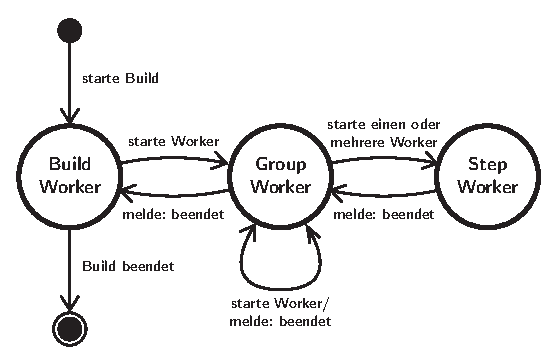
\includegraphics[width=.7\textwidth]{assets/worker_diagram}
\end{figure}

In \figref{fig:ablauf-build-prozess} ist zu sehen, wie von links nach rechts der Ablauf des Build-Prozesses geleitet wird, bis ganz rechts jeweils ein \emph{Step Worker} den eigentlichen Befehl ausführt.

Verschachtelte Worker melden ihrem übergeordneten Worker, wenn sie ihre Arbeit beendet haben. Der übergeordnete Worker kann darauf weitere Worker starten oder selbst seinem übergeordneten Worker melden, dass er beendet ist. Die Abfolge findet also rein über die Kommunikation zwischen den einzelnen Workern statt.

Auch wenn bei einem Schritt ein Fehler auftritt, wird dem übergeordneten Worker der Fehler gemeldet. Dieser beendet nun aktive Kind-Worker (insofern welche existieren) und meldet den Fehler wiederum seinem übergeordneten Worker. Somit werden Fehler im Schneeballprinzip im gesamten Prozess bekannt gegeben und strukturiert abgebrochen.

Alle Worker übermitteln über einen Websocket die aktualisierten Daten der jeweiligen Entität, damit die Änderungen auch direkt im Client angezeigt werden können.

\subsection{Entwurf der Worker}

Ein Worker ist ein Konzept in der Software-Programmierung, bei dem eine Aufgabe einem nebenläufigen Prozess zugeteilt wird. Hat ein Worker seine Arbeit beendet, ruft er einen Callback auf, um nächste Schritte auszuführen. WARP nutzt Worker zur Implementierung der Deployment-Pipeline.

Erlang (und somit auch Elixir) besitzt die Möglichkeit nebenläufige Prozesse zu starten. Diese sind keine Betriebssystem-Prozesse, sondern eigene Prozesse der Erlang VM. Durch die ressourcensparende Natur dieser Prozesse erlaubt es Erlang, eine Vielzahl von Prozessen in einer Anwendung zu verwalten. \citep[133]{Armstrong2007}

Prozesse kommunizieren untereinander mit Nachrichten und können besitzen einen Speicher bzw. Zustand (State). Diese Eigenschaften eignen sich sehr gut zur Implementierung der in \fullref{subsec:ablauf-build} beschriebenen Worker.

\subsubsection{Aufteilung in isolierte Worker}
\label{subsec:aufteilung-der-worker}

Die Worker für die Deployment-Pipeline wurden, getrennt nach ihrer Aufgabe, in verschiedene Module aufgeteilt:

\begin{description}
  \item [PipelineQueue] Eine Queue für Build-Prozesse je Pipeline.
  \item [InitWorker] Initialisiert den Build-Prozess von der Erstellung des temporären Ordners, über \texttt{git clone} und \texttt{git checkout} bis hin zum Abspeichern der Stages, Abschnitte und Schritte aus der Konfigurationsdatei.
  \item [BuildWorker] Verwaltet die Build-Entität und startet die darin befindlichen Stages.
  \item [GroupWorker] Verwaltet die Stage- oder Gruppen-Entität und startet die darin befindlichen Gruppen oder Schritte. Wie schon erwähnt, unterscheiden sich Stage und Gruppe nur darin, dass Stages immer seriell ausgeführt werden.
  \item [StepWorker] Verwaltet die Schritt-Entität und führt ihren Befehl aus.
\end{description}

\subsubsection{Kommunikation zwischen Workern}

Ein \emph{GenServer} (generic server) ist ein Elixir Prozess, der bestimmte Funktionen bereitstellt, um State im Prozess zu speichern und die Kommunikation zwischen Prozessen zu erleichtern. Er eignet sich zur Implementierung der Worker und deren Kommunikation untereinander.\footnote{vgl. https://hexdocs.pm/elixir/GenServer.html, abgerufen am 23.10.2017}

Mittels \texttt{call/3} und \texttt{cast/2} lassen sich Nachrichten an einen GenServer senden, worauf der GenServer eine Funktion ausführen kann. \texttt{call} ist eine synchrone Nachricht: nach Aufruf der Funktion wird auf eine Antwort gewartet. Im Gegensatz dazu ist \texttt{cast} eine asynchrone Nachricht, die keine Antwort erwartet.

Der GenServer nimmt diese Nachrichten über die Callbacks \texttt{handle\_\allowbreak call/3} und \texttt{handle\_\allowbreak cast/2} an.

\subsection{Implementierung eines Workers}
\label{subsec:implementierung-worker}

In diesem Kapitel wird die Implementierung eines Workers mittels GenServer anhand des BuildWorkers verdeutlicht. Zur Erinnerung: er ist für die Build-Entität verantwortlich, startet Stages und reagiert auf Nachrichten der Stage.

Ein GenServer kann mit \texttt{start/3} oder \texttt{start\_link/3} gestartet werden. Letzteres startet den GenServer unter einem \emph{Supervision Tree}. Der GenServer wird dadurch direkt beendet, wenn der aufrufende Prozess beendet wurde. Da der Build-Prozess eigenständig ausgeführt werden soll, wird \texttt{start/3} verwendet. Der Worker existiert dann so lange, bis er sich selbst beendet.

\lstinputlisting
  [caption={BuildWorker.ex: Initialisierung},
  language=elixir,
  firstline=1,
  lastline=12]
  {snippets/build-worker.ex}

Der Name \texttt{start} ist in diesem Zusammenhang irreführend: es wird zwar der Erlang Process gestartet, jedoch noch nicht der eigentliche Build-Prozess. Dies geschieht erst im nächsten Schritt (\lstref{lst:worker-run}).

Als State wird im Build-Worker die Datenbank-Entität des Builds, welche auch alle verschachtelten Gruppen und Schritte besitzt, inklusive dem Index der aktuell aktiven Stage gespeichert. Da zur Initialisierung noch keine Stage aktiv ist, wird dafür -1 genutzt. Außerdem wird die ID des Projekts gespeichert. Sie wird dazu benötigt, um Nachrichten über Websockets zu senden. Diese Nachrichten werden in einen Kanal gesendet, der über die Projekt-ID identifiziert wird.

Als Hilfsmittel stellt BuildWorker eine Funktion bereit, um den Build-Prozess nun tatsächlich zu starten. Zum Starten wird die Nachricht \texttt{:run} an den Build-Worker übermittelt.

\lstinputlisting
  [caption={BuildWorker.ex: Client-Funktionen},
  language=elixir,
  label={lst:worker-run},
  firstline=14,
  lastline=16]
  {snippets/build-worker.ex}

Mittels der beiden Funktionen \texttt{start/2} und \texttt{run/1} kann schon der BuildWorker initialisiert und gestartet werden.

\lstinputlisting
  [caption={Beispiel zum Initialiseren und Starten des BuildWorkers},
  language=elixir]
  {snippets/build-worker-start.ex}

Der GenServer muss nun auf die Nachricht \texttt{:run} reagieren. Da es sich um einen \texttt{cast/2} handelt, wird keine Antwort darauf gesendet. In diesem Callback wird die erste Stage ausgeführt.

\lstinputlisting
  [caption={BuildWorker.ex: Empfangen einer cast-Nachricht zum Starten des BuildWorkers},
  language=elixir,
  firstline=18,
  lastline=30]
  {snippets/build-worker.ex}

Die Funktion \texttt{run\_\allowbreak next\_\allowbreak stage/1} erhöht den Index der aktiven Stage und führt die entsprechende Stage als GroupWorker aus (vgl. \fullref{subsec:aufteilung-der-worker}):

\lstinputlisting
  [caption={BuildWorker.ex: Starten eines GroupWorkers für eine Stage},
  language=elixir,
  firstline=32,
  lastline=45]
  {snippets/build-worker.ex}

An dieser Stelle der Ausführung läuft ein separater Prozess, der eine Stage abarbeitet. Wir können diesen Prozess als Blackbox betrachten: was genau in ihm passiert, ist für den BuildWorker irrelevant. Wird der GroupWorker beendet, empfängt der BuildWorker eine entsprechende Nachricht, die über \texttt{handle\_\allowbreak info} empfangen wird.

\lstinputlisting
  [caption={BuildWorker.ex: Nachricht über erfolgreiches Beenden des GroupWorkers},
  language=elixir,
  firstline=47,
  lastline=63]
  {snippets/build-worker.ex}

Wenn es weitere Stages gibt, wird die erste \texttt{handle\_\allowbreak info} Funktion aufgerufen, in der die nächste Stage ausgeführt wird. Wurde die letzte Stage des Builds beendet, wird die zweite \texttt{handle\_\allowbreak info} Funktion aufgerufen und der BuildWorker beendet.

Sollte der GroupWorker mit einem Fehler beendet werden, beispielsweise weil ein Schritt nicht erfolgreich war, werden wir hierüber auch benachrichtigt. Der BuildWorker reagiert in diesem Fall darauf, dass er sich ebenfalls mit einem Fehler beendet.

\lstinputlisting
  [caption={BuildWorker.ex: Nachricht über fehlerhaftes Beenden des GroupWorkers},
  language=elixir,
  firstline=65,
  lastline=68]
  {snippets/build-worker.ex}

Direkt bevor sich der GenServers beendet, wird die Funktion \texttt{terminate/2} aufgerufen. Hier wird u.a. der Status des Builds in der Datenbank aktualisiert.

\lstinputlisting
  [caption={BuildWorker.ex: Terminieren},
  language=elixir,
  firstline=70,
  lastline=87]
  {snippets/build-worker.ex}

An einigen Stellen des Workers wird die Funktion \texttt{broadcast/2} aufgerufen. Sie sendet über Phoenix' PubSub Modul eine Nachricht über einen Websocket.

\lstinputlisting
  [caption={BuildWorker.ex: Senden einer Nachricht über einen Websocket},
  language=elixir,
  firstline=89,
  lastline=99]
  {snippets/build-worker.ex}

Die Funktion \texttt{log/2} dient zum Logging und Debugging. Auf sie wird nicht weiter eingegangen.

Die Implementierung der anderen Worker gestaltet sich ähnlich. Selbstverständlich unterscheiden sich einige Stellen und werden komplexer, beispielsweise das serielle oder parallele Ausführen von Schritten in einer Gruppe. Der Ablauf des BuildWorkers und die Kommunikation zum GroupWorker ist jedoch übertragbar auf andere Worker.
